\documentclass[a4paper,12pt]{report}
%\documentclass[twoside]{article}
%\usepackage{extsizes}
\usepackage{cmap}
\usepackage[utf8]{inputenc} %Кодировка файла 
\usepackage[T2A]{fontenc} %корректное отображение русских шрифтов
\usepackage[english, russian]{babel} %переносы слов
\usepackage{fancyvrb}
\usepackage{lmodern}

%for lcov
\usepackage{lscape} %landspace
\usepackage{float}
\usepackage{tabu}
\usepackage{booktabs}
%\usepackage{xcolor}
%\definecolor{coverage_Hi}{rgb}{0, 1, 0}
%\definecolor{coverage_Med}{rgb}{1, 1, 0}
%\definecolor{coverage_Lo}{rgb}{1, 0, 0}
%\definecolor{cov_cov}{rgb}{0.9,0.9,1}
%\definecolor{cov_diff}{rgb}{1,1,0.5}
%\definecolor{cov_nocov}{rgb}{1,0.5,0.5}
%\definecolor{cov_nop}{rgb}{0.95,0.95,0.95}
\usepackage{listings}
\usepackage{picture}

\usepackage{graphicx}

%\linespread{1.3}
\renewcommand{\rmdefault}{ftm}
%\frenchspacing

%TimeNewRoman
%\usepackage{fontspec}
%\setmainfont[Mapping=tex-text]{Times New Roman}

%Поля
\usepackage{geometry}
\geometry{left=3cm}
\geometry{right=1.5cm}
\geometry{top=2.4cm}
\geometry{bottom=2.4cm}

\usepackage{verbatim}
\usepackage{spverbatim}
\renewenvironment{lstlisting}{\spverbatim}{\endverbatim}

%\renewcommand{\labelenumii}{\arabic{enumi}.\arabic{enumii}.} %стиль нумерованных списокв

\usepackage[parentracker=true,%
  backend=biber,%
  language=auto,%
  autolang=other,%
  %citestyle=gost-numeric,%
  defernumbers=true,%
  %bibstyle=gost-numeric,%
]{biblatex}
\addbibresource{bibliography.bib}

%НАСТРОЙКИ ДЛЯ DOXYGEN

\usepackage{longtable}

\usepackage{fixltx2e}
\usepackage{calc}
\usepackage{doxygen}
\usepackage[export]{adjustbox} % also loads graphicx
\usepackage{makeidx}
\usepackage{multicol}
\usepackage{multirow}
\PassOptionsToPackage{warn}{textcomp}
\usepackage{textcomp}
\usepackage[nointegrals]{wasysym}
\usepackage[table]{xcolor}



% Font selection
%\usepackage[T1]{fontenc}
\usepackage[scaled=.90]{helvet}
\usepackage{courier}
\usepackage{amssymb}
\usepackage{sectsty}
\renewcommand{\familydefault}{\sfdefault}
\allsectionsfont{%
  \fontseries{bc}\selectfont%
  \color{darkgray}%
}
\renewcommand{\DoxyLabelFont}{%
  \fontseries{bc}\selectfont%
  \color{darkgray}%
}
\newcommand{\+}{\discretionary{\mbox{\scriptsize$\hookleftarrow$}}{}{}}

% Page & text layout
%\usepackage{geometry}
%\geometry{%
%  a4paper,%
%  top=2.5cm,%
%  bottom=2.5cm,%
%  left=2.5cm,%
%  right=2.5cm%
%}
\tolerance=750
\hfuzz=15pt
\hbadness=750
\setlength{\emergencystretch}{15pt}
\setlength{\parindent}{0cm}
\setlength{\parskip}{3ex plus 2ex minus 2ex}
\makeatletter
\renewcommand{\paragraph}{%
  \@startsection{paragraph}{4}{0ex}{-1.0ex}{1.0ex}{%
    \normalfont\normalsize\bfseries\SS@parafont%
  }%
}
\renewcommand{\subparagraph}{%
  \@startsection{subparagraph}{5}{0ex}{-1.0ex}{1.0ex}{%
    \normalfont\normalsize\bfseries\SS@subparafont%
  }%
}
\makeatother

% Headers & footers
\usepackage{fancyhdr}
\pagestyle{fancyplain}
\fancyhead[LE]{\fancyplain{}{\bfseries\thepage}}
\fancyhead[CE]{\fancyplain{}{}}
\fancyhead[RE]{\fancyplain{}{\bfseries\leftmark}}
\fancyhead[LO]{\fancyplain{}{\bfseries\rightmark}}
\fancyhead[CO]{\fancyplain{}{}}
\fancyhead[RO]{\fancyplain{}{\bfseries\thepage}}
\fancyfoot[LE]{\fancyplain{}{}}
\fancyfoot[CE]{\fancyplain{}{}}
\fancyfoot[RE]{\fancyplain{}{\bfseries\scriptsize Овчинников Владислав Александрович }}
\fancyfoot[LO]{\fancyplain{}{\bfseries\scriptsize Овчинников Владислав Александрович }}
\fancyfoot[CO]{\fancyplain{}{}}
\fancyfoot[RO]{\fancyplain{}{}}
\renewcommand{\footrulewidth}{0.4pt}
\renewcommand{\sectionmark}[1]{%
  \markright{\thesection\ #1}%
}

% Indices & bibliography
%\usepackage{natbib}
\usepackage[titles]{tocloft}
\setcounter{tocdepth}{3}
\setcounter{secnumdepth}{5}
\makeindex

% Hyperlinks (required, but should be loaded last)
\usepackage{ifpdf}
\ifpdf
  \usepackage[pdftex,pagebackref=false]{hyperref}
\else
  \usepackage[ps2pdf,pagebackref=false]{hyperref}
\fi
\hypersetup{%
  colorlinks=true,%
  linkcolor=blue,%
  citecolor=blue,%
  unicode%
}

% Custom commands
\newcommand{\clearemptydoublepage}{%
  \newpage{\pagestyle{empty}\cleardoublepage}%
}

\usepackage{caption}
\captionsetup{labelsep=space,justification=centering,font={bf},singlelinecheck=off,skip=4pt,position=top}



\title{SMTP сервер\textnumero 1}
\author{(Агеев~А.~В.)}

\begin{document}
	\maketitle

	\tableofcontents

	\addcontentsline{toc}{chapter}{Введение}
	\chapter*{Введение}
	Для функционирования компьютерных сетей, на оборудовании устанавливается программное обеспечение реализующий различные протоколы взаимодействия. Протоколы различаются по назначению. В данное время для обеспечения сети интернет используется стек протоколов TCP/IP, который состоит из протоколов выполняющий каждый свою задачу:
	\begin{itemize}
		\item Канальный уровень (например Ethernet)~--~беспечивают отправку и прием данных данных через среду передачи.
		\item Сетевой уровень (ip)~--~Канальный уровень работает с множеством устройств, которые объединены в одну группу (сеть). В данной группе устройства <<видят>> друг друга напрямую. Протоколы сетевого уровня предназанчены для обеспечения взаимодействия устройст из разных групп. Две сети объединяются маршрутизатором, а с помощью протокола сетевого уровня выплняется адресация устройств. В этом случае, между устройствами разных групп существует посредник -- маршрутизатор
		\item Транспортный уровень (TCP, UDP) -- на современном оборудовании работает множество программ, для определения того, какой программе адресованы пришедшие данные из сети, используются протоклы транспротного уровня. Их основная цель -- адресация процессов на устройстве.
		\item Прикладной уровень -- данные протоколы реализуются приложениями, которую выполняют некоторую задачу. 
	\end{itemize}

	Целью курсовой работы является реализация протокола прикладоного уровня для получения и доставки электронной почты -- Simple Mail Transfer Protocol (SMTP). А именно, части, которая выполняет прием почты и выполняет ее передачу на следующий этап -- отправку почты. 
	
	Вариант 1 предпологает многопоточную реализацию сервера.

	\chapter{Аналитический раздел}
	\section{Основные понятия протокола SMTP}

	 SMTP протокол основан на клиент-серверной архитектуре. В данном случае клиентом выступает программа, которая хочет отправить почту, а сервером является программа для приема почты. Протокол поддреживает маршрутизацию почты, то есть серверу может придти письмо, которое адресовано клиенту на другом сервере. В этом случае серверное программное обеспечение принимает роль клиента и отправлет почту другому серверу. 

	 Протокол состоит из текстовых сообщений, которые передают друг другу клиент и сервер при взаимодействии. Каждое сообщение прдеставляет из себя команду с параметрами, которые выполняются сервером. На какждую команду серверв выдает отклик. При организации надежного соединения (например посредством протокола TCP) клиент инициирует почтову транзакцию, которая состоит из последовательности команд, задающих отправителя и получателя сообщения, а так же передается содержательная часть письма. После чего клиент может завершить сеанс или начать новую почтовую транзакцию для передачи очередного письма.

	 \underline{Объекты электронной почты:} (\{Конверт; Содержимое\})
	 \begin{itemize}
	 	\item Конверт
	 	   \begin{itemize}
	 	       \item Адрес отправителя -- определяется командой \textit{MAIL FROM}, которая так же начинает почтовую транзакцию. 
	 	       \item Адрес получателей - с помощью команды \textit{RCPT TO} определяется один получатель и маршрут почты до этого получателя (в \cite{rfc2821} указано, что лучше механизм маршрутизации почты игнорировать). Данная команда может быть передана несоклько раз для указания списка получателей одного письма.
	 	       \item Дополнительные заголовки. Протокол SMTP поддреживает расширения - добавление новых заголовков и параметров к стандартным заголовкам.
	 	   \end{itemize}
	 	  \item Содержимое -- передается после отправки команды \textit{DATA}
	 	  \begin{itemize}
	 	      \item Заголовок - список полей вида <ключ>:<значение>, спецификация которых описана в \cite{rfc5322}
	 	      \item Тело сообщения - это непосредственное содержимое письма, которая представляет из себя текстовый набор данных соответсвущий спецификации форматов разны типов объектов MIME (Multipurpose Internet Mail Extensions)
	 	  \end{itemize}
	 \end{itemize}
	 Все элементы описваются с исопльзованием 7-битной кодировки US-ASCII, но это ограничение может быть снято с использованием расширения протокола \textit{8BITMIE}. Так же возможно приминение кодировки BASE64 позволяющей представить любую последовательность байт в текстовой кодировке US-ASCII.
	
	 \underline{Получатель и отправитель:}
	 
	 Протокол SMTP работает в 2 стороны. Получателем и отправителем может выступать как почтовая служба на сервере так и клиентское программное обеспечение. В протоколе выделяются следующие понятия:
	 \begin{itemize}
	     \item Клиент -- Отправлющая сторона в текущей почтовой транзакции.
	     \item Сервер -- Принимающая сторона в текущей почтовой транзации.
	     \item Агент доставки почты (Mail Transfer Agent, MTA)~-- Клиент и сервер SMTP обеспечивающее почтовый трансопртный сервис.
	     \item Пользовательский почтовый агент (Mail User Agent, MUA)~-- Программное обеспечение выступающее в качетсве исходных отправителей и конечных получателей почтовых сообщений
	 \end{itemize}
	 $$MUA\rightarrow MTA \rightarrow MTA \rightarrow MUA$$
	 
	 \underline{Типы агентов SMTP:}
	 
	 \begin{itemize}
	     \item Система отрпавки (originator) -- Вносит сообщение в среду передачи данных, в котором находится транспортный сервис.
	     \item Система доставки (delivery) -- Принимает почту от транспортного серивса и передает ее пользовательскому агенту или размещает ее в хранилище.
	     \item Транслятор (relay) -- Получает почту от клиента и передает ее другому серверу.
	     \item Шлюз (gateway) -- Система получающие письма от одной транспортной среды и передающие письма сереверу находящейся в другой транспортной среде.
	 \end{itemize}
	 
	 
	 \section{SMTP сеанс}
	 
	 При подключении клиента к серверу начинается SMTP сеанс, в течении которого выполняется взаимодействие клиента и сервера по доставки писем.
	 \begin{enumerate}
	     \item Инициирование соединения 
	     
	     Клиент: создает соединение с сервером
	     
	     Сервер: Отправляет отклик
	     \begin{itemize}
	         \item 220 в случае готовности
	         \item 554 в случае отказа в SMTP сервисе
	     \end{itemize}
	     \item Инициирование клиента (сеанса)
	     
	     Клиент: передает команду \textit{HELO/EHLO}. \textit{HELO} - содание SMTP сеанса. \textit{EHLO} - создание SMTP сеанса с поддержкой расширений протокола (Extend Hello).
	     
	     Сревер: Отрпавляет отклик 250. Если была отправлена команда \textit{EHLO}, то сервер так же возращает список расширений, который он поддерживает (расширения далее не рассматриваются)
	     
	     \item Почтовая транзакция (Транзакцию нельзя сделать вложеной в другую транзакцию)
	     \begin{enumerate}
	         \item \label{item:mail_transaction} Начало транзакции
	         
	         Клиент: Отправлет команду \textit{MAIL FROM}. Команда говорит о запуске новой почтовой транзакции и передает адрес отправителя. Если в процессе передачи возникнет ошибка, на этот адрес будет отправлено уведомление. Обратный адрес может быть пустым
	         
	         Сервер: Отклик 250
	         
	         \item Определение спика получателей
	         
	         Для определение списка получателей клиент отправлет несколько команд \textit{RCPT TO}, на каждую из которых сервер отправляет отклик 250.
	         
	         Если команда \textit{RCPT TO} отправлена до начала почтовой транзакции, то сервер отправлет отклик 503
	         
	         \item Передача тела письма 
	         
	         Клиент: Отправлет команду \textit{DATA} 
	         
	         Сервер: отправлет отклик 354, что свидетельствует о том, что сервер готов принимать содержимое письма
	         
	         Клиент: Отрпавлет все почтовые данные. После завершения отправки тела письма, клиент должен отправить точку на отдельной строке (<CRLF>.<CRLF>~--~послеовательность окончания данных письма)
	         
	         Сервер: Должен воспринимать все присилаемые данные, как тело письма. Как только он получает последовательность конца данных (<CRLF>.<CRLF>) сервер должен инициировать процесс доставки письма. А клиенту отправить отклик 250
	     \end{enumerate}
	     
	     \item Завершение сеанса или новая транзакция
	     \begin{itemize}
	         \item Если клиент желает завершить работу с сервером, то он должен послать команду \textit{QUIT}, на которую сервер должен ответить откликом 221 и закрыть соединение
	         \item Если клиент желает продолжить работу с сервером, то он должен создать новую почтовую транзакцию. Для этого необходимо перейти на шаг \ref{item:mail_transaction}
	     \end{itemize}
	 \end{enumerate}
	 
	 \underline{Дополнительные команды:}
	 \begin{enumerate}
	     \item \textit{VRFY} -- проверка пользователей на сервере
	     \item \textit{EXPN} -- проверка адресов рассылки
	     \item \textit{RSET} -- прерывание текущей почтовой транзакции. Отклик сервера: 250
	     \item \textit{HELP} -- справка по команде
	     \item \textit{NOOP} -- пустая команда, сервер всегда возращает отклик 250
	 \end{enumerate}
	
	 \section{Синтаксис команд}\label{section:smtp_syntax}
	 \begin{verbatim}
ehlo = "EHLO" SP Domain CRLF
helo = "HELO" SP Domain CRLF
ehlo-ok-rsp  = ("250" domain [SP ehlo-greet] CRLF)
              | ("250-" domain [SP ehlo-greet] CRLF
              | *("250-" ehlo-line CRLF)
              | ("250" SP ehlo-line CRLF)

ehlo-greet = 1*(%d0-9 / %d11-12 / %d14-127)
ehlo-line = ehlo-keyword *( SP ehlo-param )
ehlo-keyword = (ALPHA / DIGIT) *(ALPHA / DIGIT / "-")
ehlo-param   = 1*(%d33-127)
"MAIL FROM:" ("<>" / Reverse-Path) [SP Mail-parameters] CRLF
"RCPT TO:" ("<Postmaster@" domain ">" /
           "<Postmaster>" / Forward-Path) 
           [SP Rcpt-parameters] CRLF
"DATA" CRLF
"RSET" CRLF
"VRFY" SP String CRLF
"EXPN" SP String CRLF
"HELP" [ SP String ] CRLF
"NOOP" [ SP String ] CRLF
"QUIT" CRLF
Reverse-path = Path
Forward-path = Path
Path = "<" [ A-d-l ":" ] Mailbox ">"
A-d-l = At-domain *( "," A-d-l )
At-domain = "@" domain
Mail-parameters = esmtp-param *(SP esmtp-param)
Rcpt-parameters = esmtp-param *(SP esmtp-param)
esmtp-param     = esmtp-keyword ["=" esmtp-value]
esmtp-keyword   = (ALPHA / DIGIT) *(ALPHA / DIGIT / "-")
esmtp-value     = 1*(%d33-60 / %d62-127)
Keyword  = Ldh-str
Argument = Atom
Domain = (sub-domain 1*("." sub-domain)) / address-literal
sub-domain = Let-dig [Ldh-str]
address-literal = "[" IPv4-address-literal / 
                      IPv6-address-literal /
                      General-address-literal "]"
Mailbox         = Local-part "@" Domain
Local-part      = Dot-string / Quoted-string
Dot-string      = Atom *("." Atom)
Atom            = 1*atext
Quoted-string   = DQUOTE *qcontent DQUOTE
String          = Atom / Quoted-string
IPv4-address-literal    = Snum 3("." Snum)
IPv6-address-literal    = "IPv6:" IPv6-addr
General-address-literal = Standardized-tag ":" 1*dcontent
Standardized-tag        = Ldh-str
Snum                    = 1*3DIGIT
Let-dig                 = ALPHA / DIGIT
Ldh-str                 = *( ALPHA / DIGIT / "-" ) Let-dig
IPv6-addr               = IPv6-full / IPv6-comp / IPv6v4-full / IPv6v4-comp
IPv6-hex  = 1*4HEXDIG
IPv6-full = IPv6-hex 7(":" IPv6-hex)
IPv6-comp = [IPv6-hex *5(":" IPv6-hex)] "::" [IPv6-hex *5(":"IPv6-hex)]
IPv6v4-full = IPv6-hex 5(":" IPv6-hex) ":" IPv4-address-literal
IPv6v4-comp = [IPv6-hex *3(":" IPv6-hex)] "::"
              [IPv6-hex *3(":" IPv6-hex) ":"] IPv4-address-literal
	 \end{verbatim}

	 \section{Архитектура -- Цикл событий}

    Для реализации поддержки многопоточности используется Циклы событий, смысл которого заключается в том, что существует бесконечный цикл, ожидающий событий на сокете через системный вызов poll. Данный цикл работает в отдельном потоке. Так же существует несколько других потоков, которые называются работниками. Они выполняют обработку возникающих событий. Сущесвует следующее множество событий, для которых можно назначить функцию обработчик:
    \begin{enumerate}
        \item Событие <<Подключился клиент>>
        \item Событие <<Выполнено чтение из сокета>>
        \item Событие <<Выполнена запись в сокет>>
        \item Событие <<Истек таймер>>
        \item Событие <<Сокет был закрыт>> (запрос о закрытие сокета со строны сервера)
    \end{enumerate}
    
    Основным преймуществом данного подхода является том, что все потоки разделают одно адресное пространство -- быстрое взаимодействие между ними. В отличие от многопроцессной архитектуры, в которой имеются накладные расходы на обмен информацией между процессами, так необходимо использовать соответсвующие системные вызовы, что заставлет процессор переключаться в режим ядра. Хотя постоянное использование механизмов синхронизации, при доступе к разделяемым ресурсам, так же замедляет работу приложения. А недостатком многопотончой архитектуры является ненадежность -- если в одном из потоке произойдет критическая ошика (например \textit{SIGFAULT}), то будет уничтожен процесс, соответсвенно все потоки приложения немедленно завершат свою работу. В этом случае многопроцессная архитектура имеет преймущество в виде надежности. Критическая ошибка в одном процессе не затрагивает другие процессы. Так же можно реализовать отдельный процесс, который будет выполнять мониторинг состояний рабочих процессов (watchdog-процесс), и вслучае экстренного завершения одного из процессов, watchdog-процесс должен будет выполнить восстановление завершившегося процесса (выполнение его повторного запуска). 
    
    Менеджер событий реализуется посредством струтуры \textit{event\_loop}, запускаемый функцией \textit{el\_open} в отдельном потоке. Структуре сопутсвуют функции для регистрации обработчиков на события. Регистрация на событие одноразовое, т.е. после вызова обработчика события, данный обработчик не будет реагировать на данное событие -- его необходимо заново зарегистрировать. 
    
    Рабочим потокам, которые будут обрабатывать события, необхоимо в цилке вызывать функцию \textit{el\_run}, функция выполняет обработку одного события и завершает работу. Если в момент вызова, отсутсвовали какие либо события, то функция немедленно возращает управление, сообщая об отсутсвии событий в возращаемом статусе. Пример работы цикла событий показан на диаграмме последовательности (рис. \ref{fig:EventLoopSequence}). 

Функция \textit{el\_run} только обрабатывает событие, не предполагает создание потока. Для реализации многопоточной обработки был реализована вспомогательная структура \textit{thread\_pool}, используюя функции которой создаются потоки. Внутри каждого потока в бесконечном цикле выполняется вызов функции \textit{el\_run}. 
    

    
    Для корректного завершения работы, бесконечные циклы, на самом деле проверяют условие <<Необходиом ли дальше работать>> (циклы логически бесконечны, так как они работают до тех пор, пока работает приложение). Для корректного заврешния работы программы, используется обработчик сигналов, который регистрируется в операционной системе. Если приходит сигнал \textit{SIGTERM} или \textit{SIGINT}, то обработчик вызывает функцию \textit{el\_stop}, которая изменяет флаг работы цикла событий с true на false. Таким образом на очередной проверки условия работы цикла всеми потоками, учавствующие в цикле событий, будет произведен выход. Все потоки завершат свою работу и приложение остановится.


	\begin{figure}[H]
		\centering
		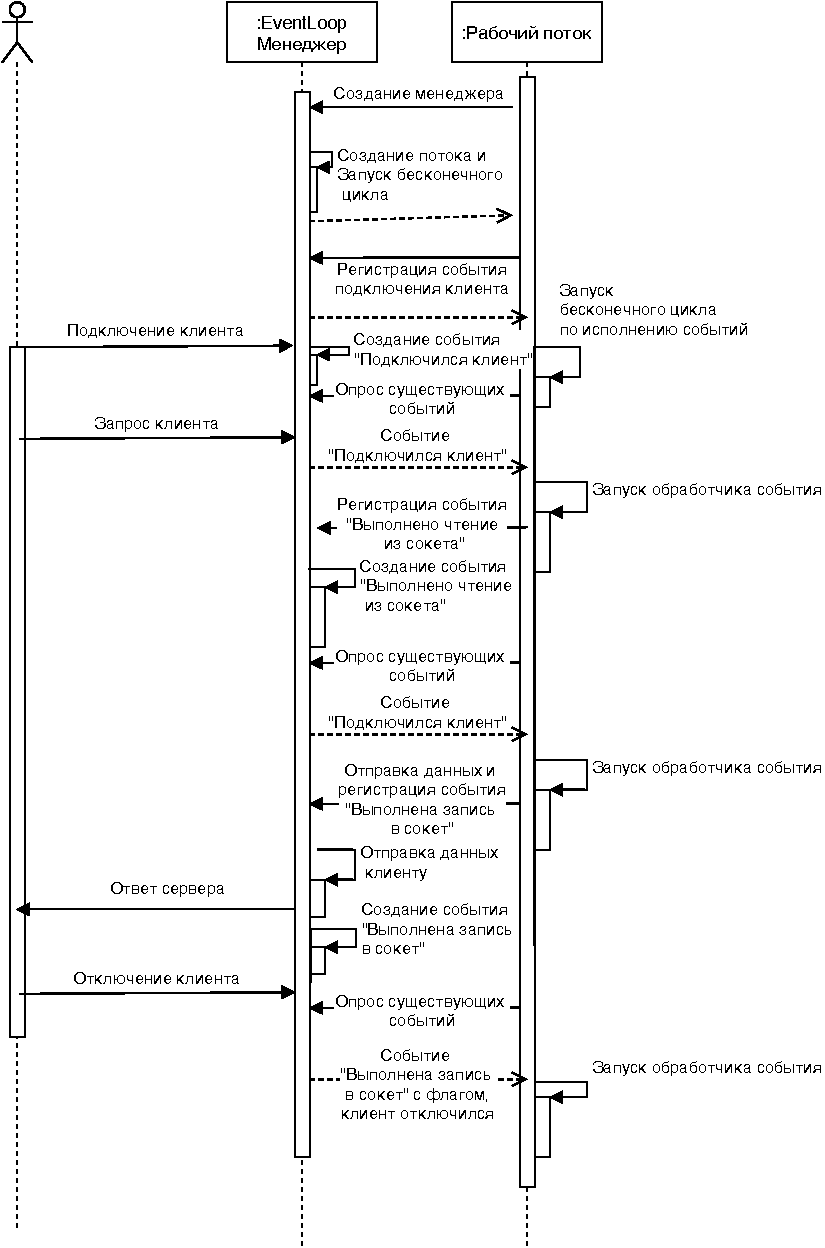
\includegraphics[width=0.8\textwidth]{./resource/SequenceDiagram_EventLoop.pdf}
		\caption{ Диаграмма последовательности цикла событий сервера, описывающая подключение клиента, который отправлет запрос, ожидает ответ, а потом отключается. При отключении клиента, выставлется соответсвующий флаг, который обрабатывается в обработчике чтения из сокета или записи в сокет.} \label{fig:EventLoopSequence}
	\end{figure}


 \chapter{Конструкторский раздел}

 \section{Реализаця протокола SMTP}
    
    \begin{figure}[h]
	\centering
	\includegraphics[width=\textwidth]{./include/smtp_fsm.pdf}
	\caption{Конечный автомат протокола SMTP}
	\label{fig:smtp_fsm}
\end{figure}

    
    Обработка сеанса протокола SMTP выполняется на основе цикла событий. Для реализации конечного автомата и связанных с ним действий была реализована стркуктура \textit{smtp\_state}, которая содержит в себе конечный автомат, созданный посредством утилиты \textit{autofsm}. На рисунке \ref{fig:smtp_fsm} показан конечный автомат, который описан в файле \textit{smtp-states.def}. Овалами обозначены состояния, а метки ребер это команды. Таким образом каждая команда выполняет изменение состояния. Существует ряд меток, которые как команды, отсутсвуют в протоколе. 
    \begin{itemize}
        \item \textit{TEST} -- это метка обозначает следующие команды: \textit{VRFY}; \textit{EXPN}; \textit{HELP} \textit{NOOP}; 
        \item \textit{READ} -- это любая последовтаельность символов кроме \textit{.\textbackslash{}r\textbackslash{}n} (точка на отдельной строке).
    \end{itemize}
    
    \underline{Состояния конечного автомата (рис. \ref{fig:smtp_fsm})}
    \begin{enumerate}
        \item init -- Начальное состояние, в котором находится соединение, когда клиент только подлкючился к серверу
        \item client init -- Состояние инициализированного smtp сеанса. В него выполняется переход после отправки команды \textit{HELO} или \textit{EHLO}
        \item begin transaction -- инициализация почтовой транзакции, которая происходит, когда клиент отправлет команду \textit{MAIL FROM}
        \item transaction -- определение списка получателей, с помощью команды \textit{RCPT TO}
        \item  read data -- получение сервером тела письма. Данная стадия запускается командой \textit{DATA} и продолжается до тех пор, пока не будет получена последовательность конца данных (точка на отдельной строке: \textit{.\textbackslash{}r \textbackslash{}n}). На рисунке обозначена меткой END
        \item done -- завершение сенаса клиента с сервером. Отправлется команда \textit{QUIT} и сервер закрывает соединение.
    \end{enumerate}
    
    Автомат описывает только корректную последовательность команд, но если в некотором состоянии будет передана команда, которая не определена конечным автоматом, то состояние не изменится, а сервер сформирует отклик с кодом 503, означающий что клиент ввел неподходяющую команду (некорректная последовательность команд).
    
    Для обработки команд SMTP протокола, синтаксис которых описан в разедел \ref{section:smtp_syntax}, использовались регулярные выражения. Регулярные выражения описаны в следующем листинге:
    \input{./include/regex}
    
    \section{Maildir -- формат хранения писем в файловой системе}
    Для хранения почты, получаемой сервером посредством почтовой транзакции, используется файловая система. Используемая струтктура каталогов взята из спецификации \textit{MAILDIR}, которая описана в \cite{dovecot_maildir, qmail_maildir}. Формат maildir имеет следующую структуру каталогов:
    \begin{verbatim}
        - maildir_root
        |
        |- user_path
        |    |- cur
        |    |- tmp
        |    |- new
        |
        |- user2_path
        |    |- cur
        |    |- tmp
        |    |- new
    \end{verbatim}
    Где maildir\_root - кореньевая папка. user\_path, user2\_path - каталоги пользователей текущей почтовой службы. cur, tmp, new - папки содержащие письма. 
    new - сюда попадают письма новые письма, которые пользователь не прочитал. cur - письма просмотренные пользователем. tmp - пиьсма находящиеся на стадии доставки, необходимость этой папки заключается в том, что запись данных в файл не является атомарной операцией. Если этой папки не будет то при создании файла, например в папке new, может произойти так, что программа для чтения локальной почты, попытается открыть этот новый файл, а программа доставки почты еще не успела туда записать данные. По этому используется каталог tmp для исключения таких случаев. Пока данные записываются в файл, тот находится в папке tmp, как только письмо полностью записано в файл, то программа доставки писем переносит этот файл в каталог new.
    
    При создании новых файлов писем, им необходимо давать имена. Для создания уникального имени формат MAILDIR трактует слудющие правила:
    \begin{verbatim}
        <pid><sender_mailbox><timestamp><random_value>
    \end{verbatim}
    Где <pid> - идентификатор процесса, выполняющий доставку почты; <sender\_mailbox> - адрес электронной почты отправителя письма;  <timestamp> - время UNIX; <random\_value> - случайное целое число.
    
    Поскольку формат MAILDIR разработан для доставки локальной почты, а по заданию необходимо обрабатывать и глобальную почту (почту адресованную пользователям на других серверах), то формат MAILDIR был модифицирован следующим образом: 
        
        \begin{verbatim}
        - maildir_root
        |
        |- user_path
        |    |- cur
        |    |- tmp
        |    |- new
        |
        |- user2_path
        |    |- cur
        |    |- tmp
        |    |- new
        |
        |- .OTHER_SERVERS
        |    |-server1.ru
        |    |    |- tmp
        |    |
        |    |-server2.com
        |    |    |-tmp

    \end{verbatim}
    Модификация maildir добавляет папку \textit{.OTHER\_SERVERS}, в которой расположены папки целевых серверов. Внутри которых складываются письма предназанченные внешним (соответсвующим) серверам. Отсутсвует папка new, но присутствует папка tmp для решения проблемы <<отправки еще недоставленного письма>>. Полностью записанный файл с письмом перемещается из папки tmp в корневую папку внешнего сервера. После того, как письмо будет доставлено внешнему серверу, файл письма должен быть удален для предотвращения повторной доставки. Так же изменен формат создания уникального имени файла:
    \begin{verbatim}
        <timestamp>_<random_value>
    \end{verbatim}
    Использую такой формат, нельзя определить по файлу от кого письмо и кому адресовано, по этому при записи письма  к телу письма дописываются дополнительные заголовик, с помощью которых отправляющая программа сможет определить адресата и адресанта:
    \begin{verbatim}
        X-Postman-From: <mailbox>
        X-Postman-Date: <timestamp>
        X-Postman-To: <mailbox> [, <mailbox> [...]]
        <пустая строка (\r\n)>
        <тело письма полученное во время почтовой транзакции>
    \end{verbatim}
    
    Обработка данной структуры в файловой системы реализовано с помощью класса \textit{maildir}. Дописыване дополнительных заголовков реализовано в обработчике почтовой транзакции, а не внутри класса \textit{maildir}.

\section{Логика программы}

	\begin{figure}[H]
		\centering
		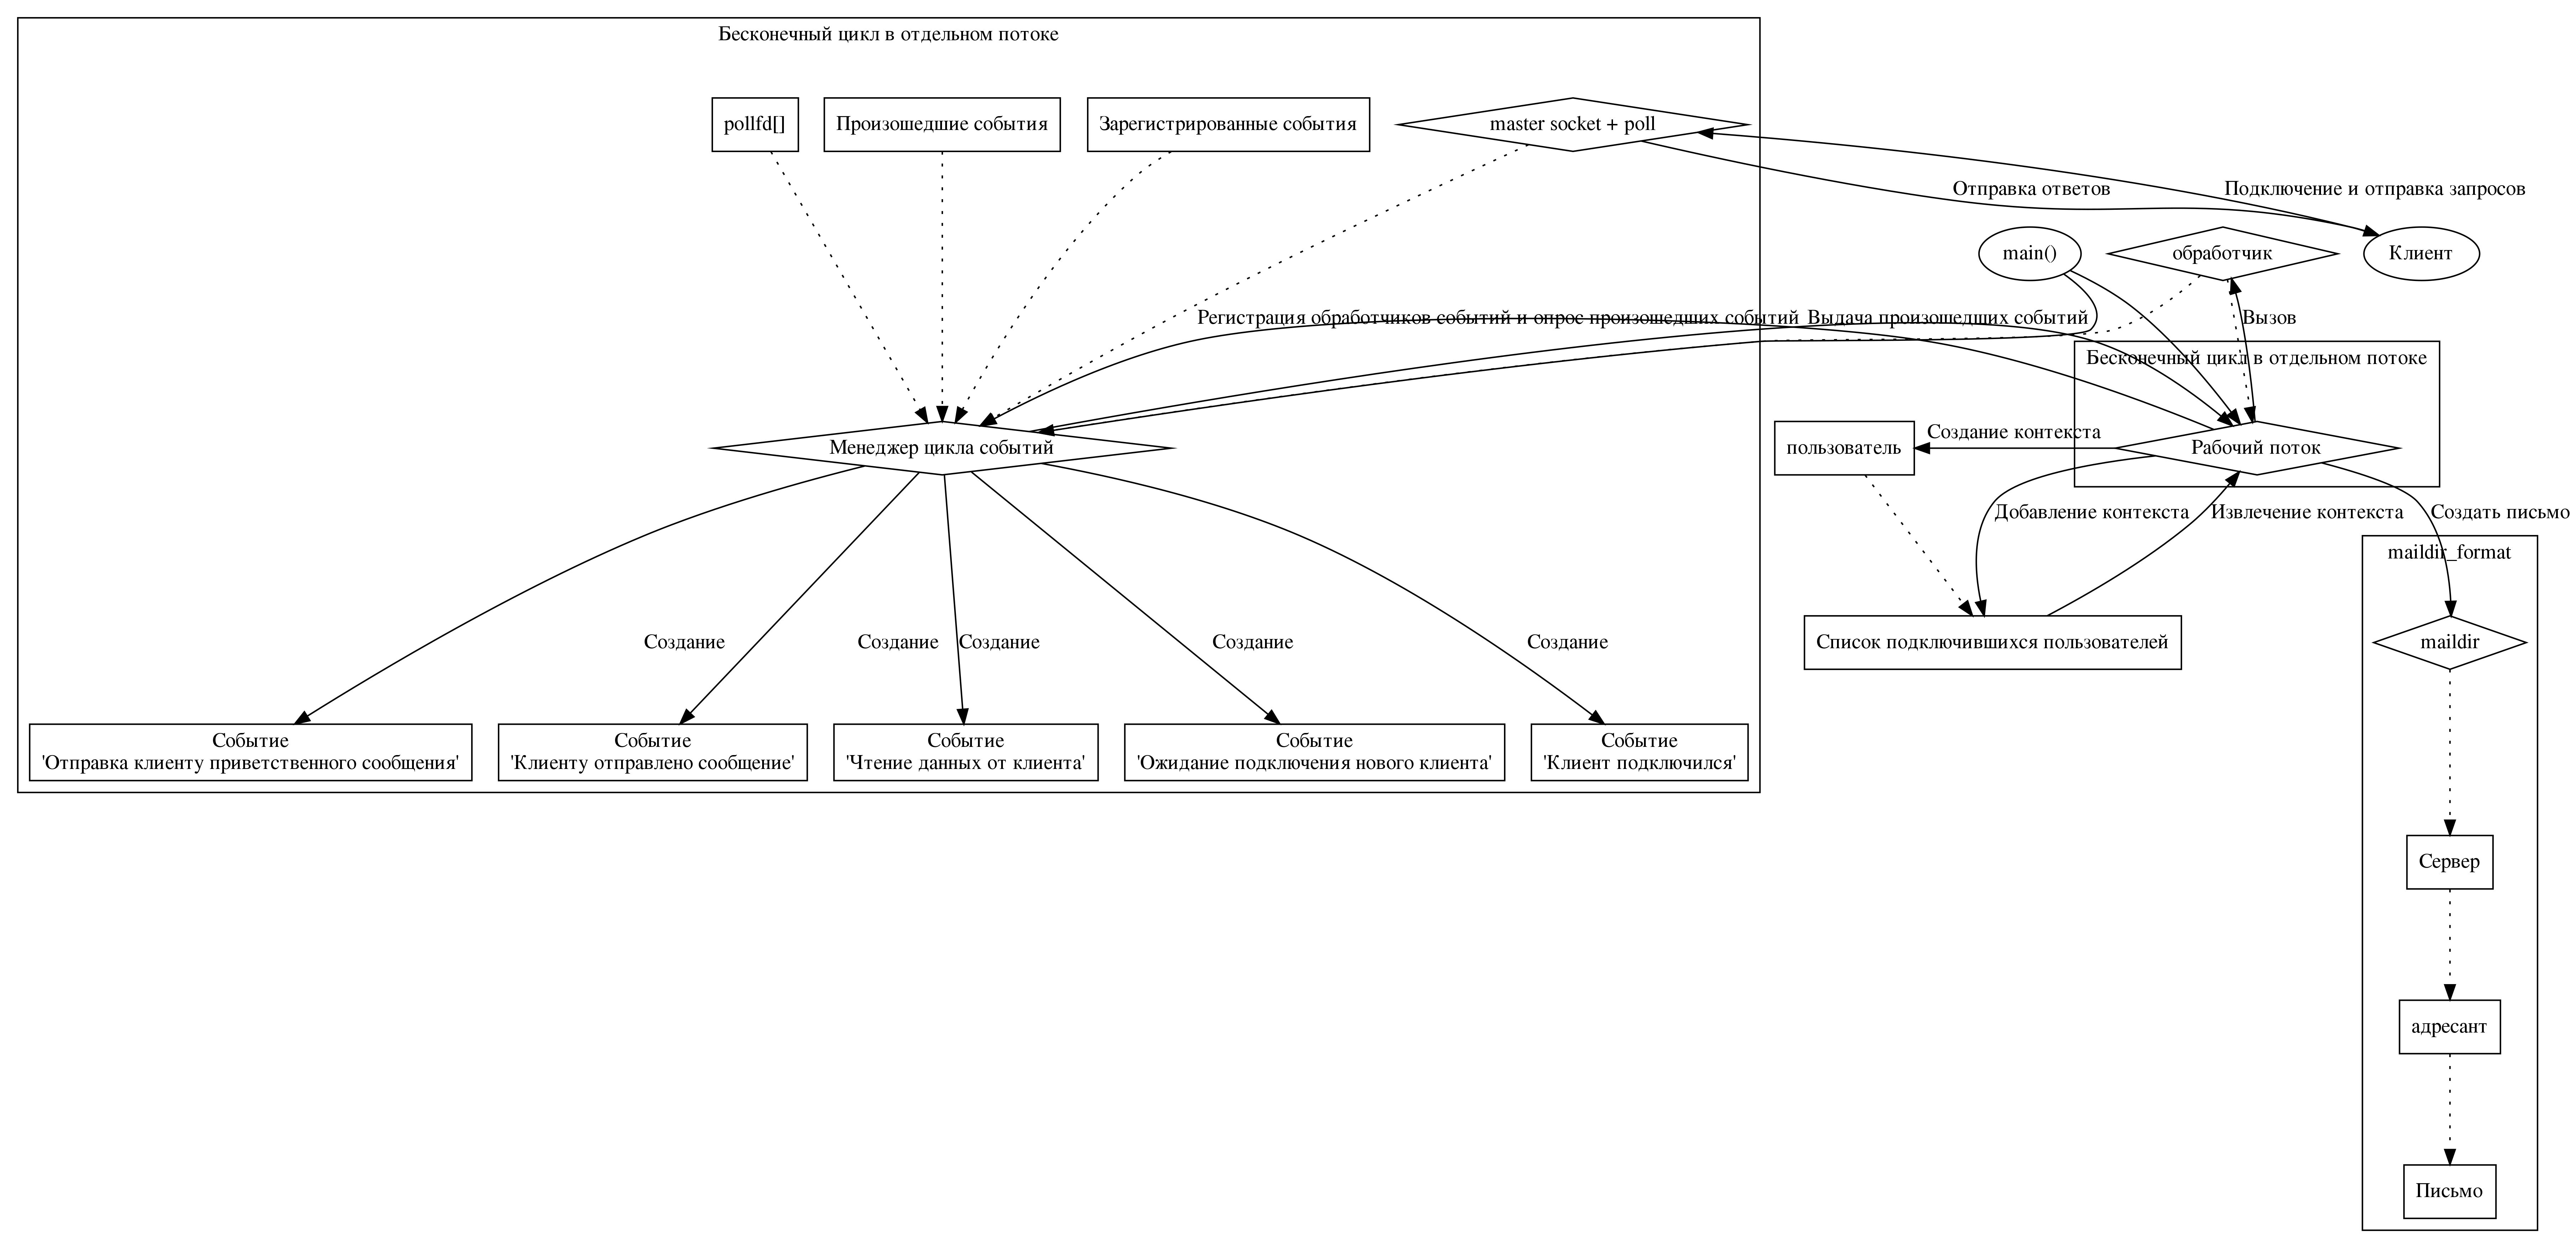
\includegraphics[width=\textwidth]{./resource/logic.png}
		\caption{Упращенная диаграмма взаимодействия модулей. EventLoop осуществлет обработку подключений. Рабочий поток осуществляет вызов обработчиков событий, которые EventLoop создает. Модуль mailidr обеспечивает сохраенние писем в файловой ситемы в соответсвующем формате} \label{fig:ProgLogic}
	\end{figure}

	Программа написана с использованием Объектно Ориентированной парадигмы, хотя язык С напрямую ее не поддерживает. Для описания объектов используются структуры, для которых принято слоедующее соглашение:
	\begin{itemize}
		\item Поле считается приватным (private) если его название начинается с префика pr или \_ (нижнее подчеркивание). Защищенные (protected) поля не используются.
		\item Функция (метод структуры) считается приватным, если его название начинается с префикса pr или \_ (нижнее подчеркивание)
	\end{itemize}
	Так же используется некоторое подобие наследования. Наследование реализуется двумяспособаи.

	 Первый способ: Создается общая структура для всех наследников, которая содержит тип наследника. Контейнер содержит указатель типа общего класса. При извлечении объекта из контейнера и перед обращением к его полям, по полю типа объекта определяется тип наследника, а затем выполняется соответсвующее приведение типов. Данный способ используется в цикле событий.

	 Второй способ: Создается базовая структура, которая содержит в себе описатель фактического типа объекта и поля заполнители, которые предназначены для того, чтобы родитель и все его потомки занимали одинаковое пространство в памяти на стеке. Что позволяет вместо указателей на структуры в контейнерах хранить сами струтктуры. По полю тип, определяется фактический тип объекта и выполняется приведение типов при обращении к объетку. Данный метод используется в реализации логирования, для хранения в массиве методов вывода лога (на экран или в файл).


	
	Работа программы начинается с того, что выполняется чтение конфигурационного файла, пример которого представлен в следующем листинге. 

	\VerbatimInput{../../resource/config2.cfg}

	Чтение конфигурационного файла реализовано посредством бибилотеки \textit{libconfig}. \textit{server\_config\_init} реализует логику для заполнения глобальной структуры \textit{server\_configuration} содержащая все необходимые объекты для работы сервера. 

	 После инициализации данной структуры, выполнятся создание экземпляра класса цилка событий (event\_loop с помощью функции el\_init), затем создается сокет, выполняющий прослушивание порта (master\_socket, функция make\_server\_socket). Далее для данного сокета выполняется регистрация обрабтчика события подключения нового клиента. (обработчик - функция handler\_accept) Регистрация выполняется для конкретного экземлпяра структуры event\_loop. Таким образом, когда клиент выоплнит подключение к серверу, будет вызван зарегистрированный обработчик, в который будет передедан экземпляр event\_loop, серверный сокет и клиентский сокет. На рисунке \ref{fig:handlers} показана логика взаимодействия разных видов обработчиков между собой. Это взаимодействие существует, поскольку все событя, кроме таймеров и подключения новых клиентов являются одноразовыми и их необходимо заново регистрировать.

	 	\begin{figure}[H]
		\centering
		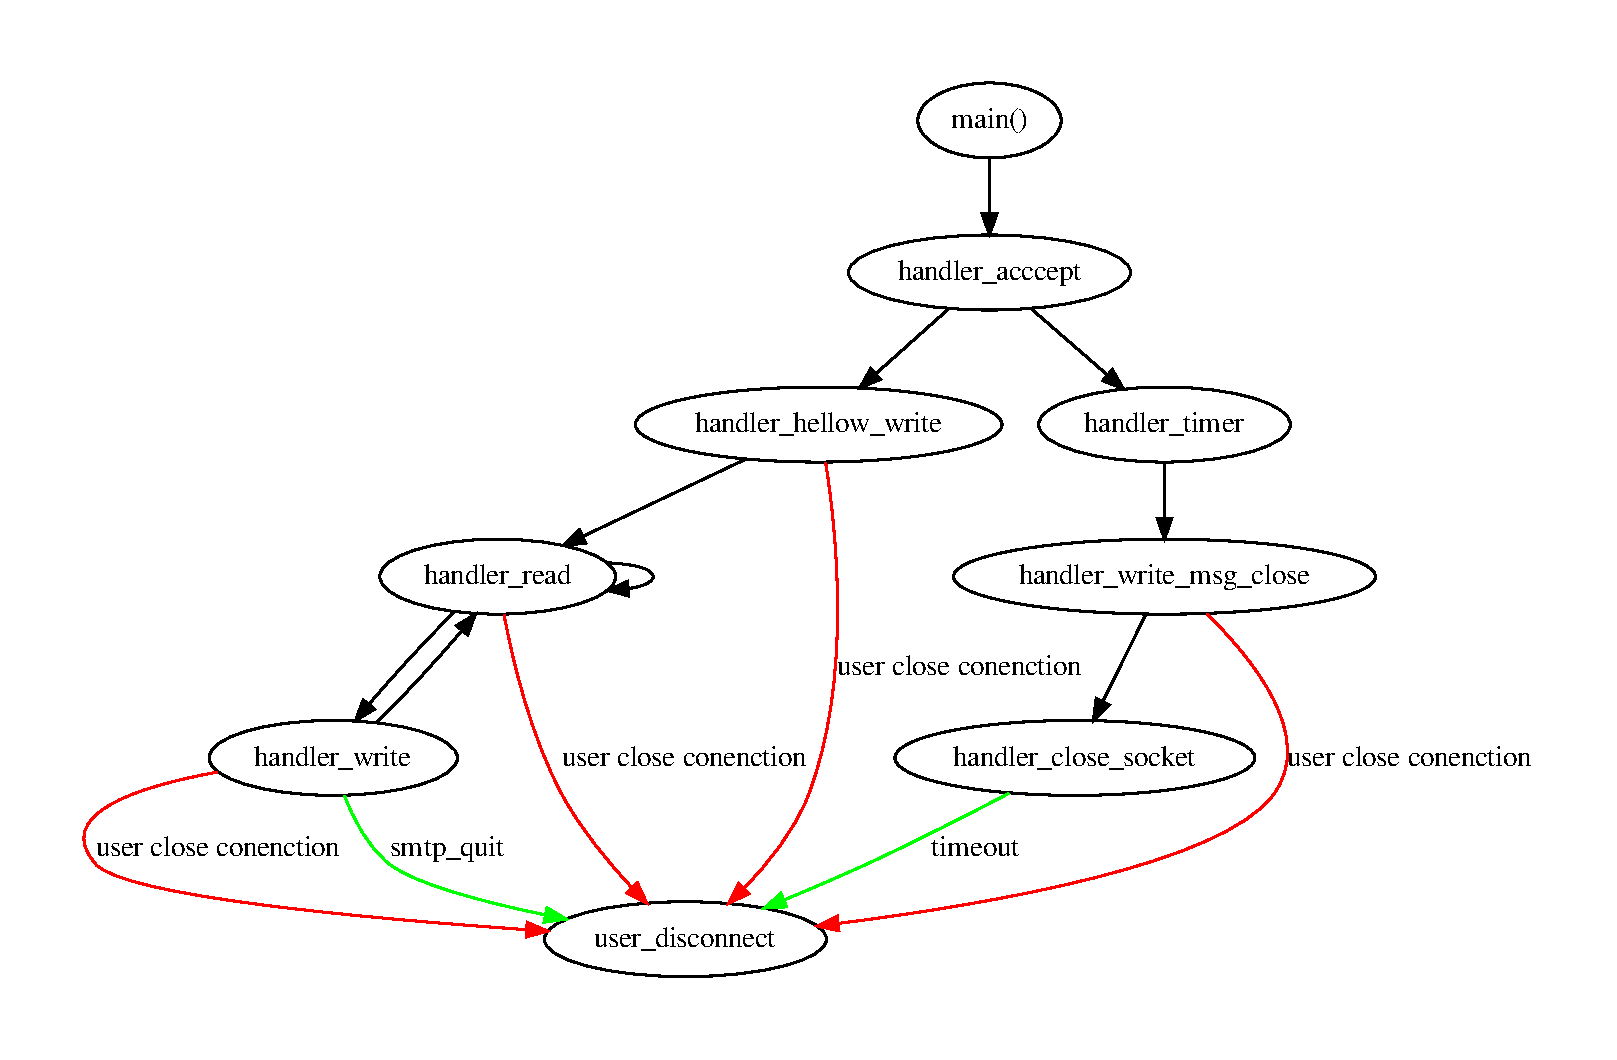
\includegraphics[width=\textwidth]{./resource/handlers.pdf}
		\caption{Псоледовательность выполнения обработчиков событий. функции main и user\_disconnet не явлются обработчиками в смыле event\_loop, а явлются началом и концом работы.  Стрелками обозначены возможные переходы во время работы. При этом две образовавшеся ветки (выходящие из узла handler\_accept), работают одновременно. Так как event\_loop многопоточный. Зеленая стрелка означает корректный переход в конечное состояние, а красная -- переход по возникшей ошибке} \label{fig:handlers}
	\end{figure}

	Жизненый цилк взаимодействия клиента с сервером начинает с обработчика handler\_accept, который вызывается при подключении клиента к серверу. В этот момент регистрируются обработчики для отправки приветсвенного сообщения от сервера и таймер на ождинаие команд от пользователя. Левая ветка, описывает переходы между обработчиками во время передачи команд от клиента к серверу, и передачи откликов от сервера клиенту. Правая ветка следит за тем, что бы клиент успевал отправлять команды в отведенный промежуток времени. Но клиент, может выполнить отключение от сервера нарушая протокол SMTP (самостоятельно или по ошибке, такие переходы обозначены, красной стрелкой). Завершение работы с клиентом выполняется в функции client\_disconnect, в которой выоплняется очищение всех ресурсов, выделенных во время работы с клиентом.

	Поскольку протокол smtp имеет состояние, то для каждого активного подключения его необходимо хранить. Для реализации хранения состояния протокола исопльзуется структура \textit{user\_context}, котоаря содержит буфер чтения, записи, состояние протокола smtp, сокет, по которому выполняется общение и адрес клиента. 

	Так как сервер многопоточный, то необходимо выполнять защиту доступа к контекстам пользователей. Для этого был реализован потокобезопасный список контекстов пользователей \textit{users\_list}. Данный список защищает 1 мьютекс. В этом случае использование грубой синхронизации сводит на нет все преймущества использования многопоточности, по этому применяется следующий трюк. Исходя из предположения, что одновременно одного пользователя может обрабатывать 1 поток (обработка таймеров нарушает это предположение, о них будет написано далее). Таким образом, доступ к контексту пользователя описывается следующими шагами:
	
	\begin{enumerate}
		\item Блокируем мютекс.
		\item \label{item:user_find} Ищем контекст пользователя по сокету, перебирая подряд элементы списка.
		\item  Если пользователя нашли, то удаляем его из списка, но самого пользвателя оставляем. 
		\item Разблокируем мютекс.
		\item Возвращаем пользователя. 
	\end{enumerate}

	Если на шаге \ref{item:user_find} пользователь не был найден, то возвращаем NULL.
	
	При получении пользователя из защищенного списка, возращается не сам контекст, а обертка \textit{user\_accessor}, которая предназначена для того, чтобы после окончания работы с контекстом, его можно было обратно вернуть в список контекстов. 

	Событие таймера является асинхронным и зависит только от активности клиента. Их обработка выполняется в некотором рабочем потоке, и тогда может возникнуть ситуация: <<Один рабочий поток, обрабатывает запрос клиента, а другой поток начал обрабатывать событие таймера>>, таким образом возникнет проблема: поток обрабатывающий таймер, не сможет найти контекст пользователя, так как пока он обрабатывается в другом обработчике, он является извлеченным из списка. Для решения данной проблеммы структура описывающая таймеры была вынесена в отдельную структуру <<список таймеров>> \textit{timers\_t}, которая предоставляет функции для добавления и удаления таймера, проверки <<истек ли таймер для конкретного сокета>>, обновление значения для таймера. Для доступа к конкретному таймеру используется грубая синхронизация.

	Для компилирования сервера, тестов и отчета используется утилита make. Структура проекта показана на рисунке \ref{fig:make_server}. Граф вызова всех функций, которые реализуют всю вышеописанную логику показан на рисунке \ref{fig:cflow}.

	\begin{figure}[H]
	\centering
	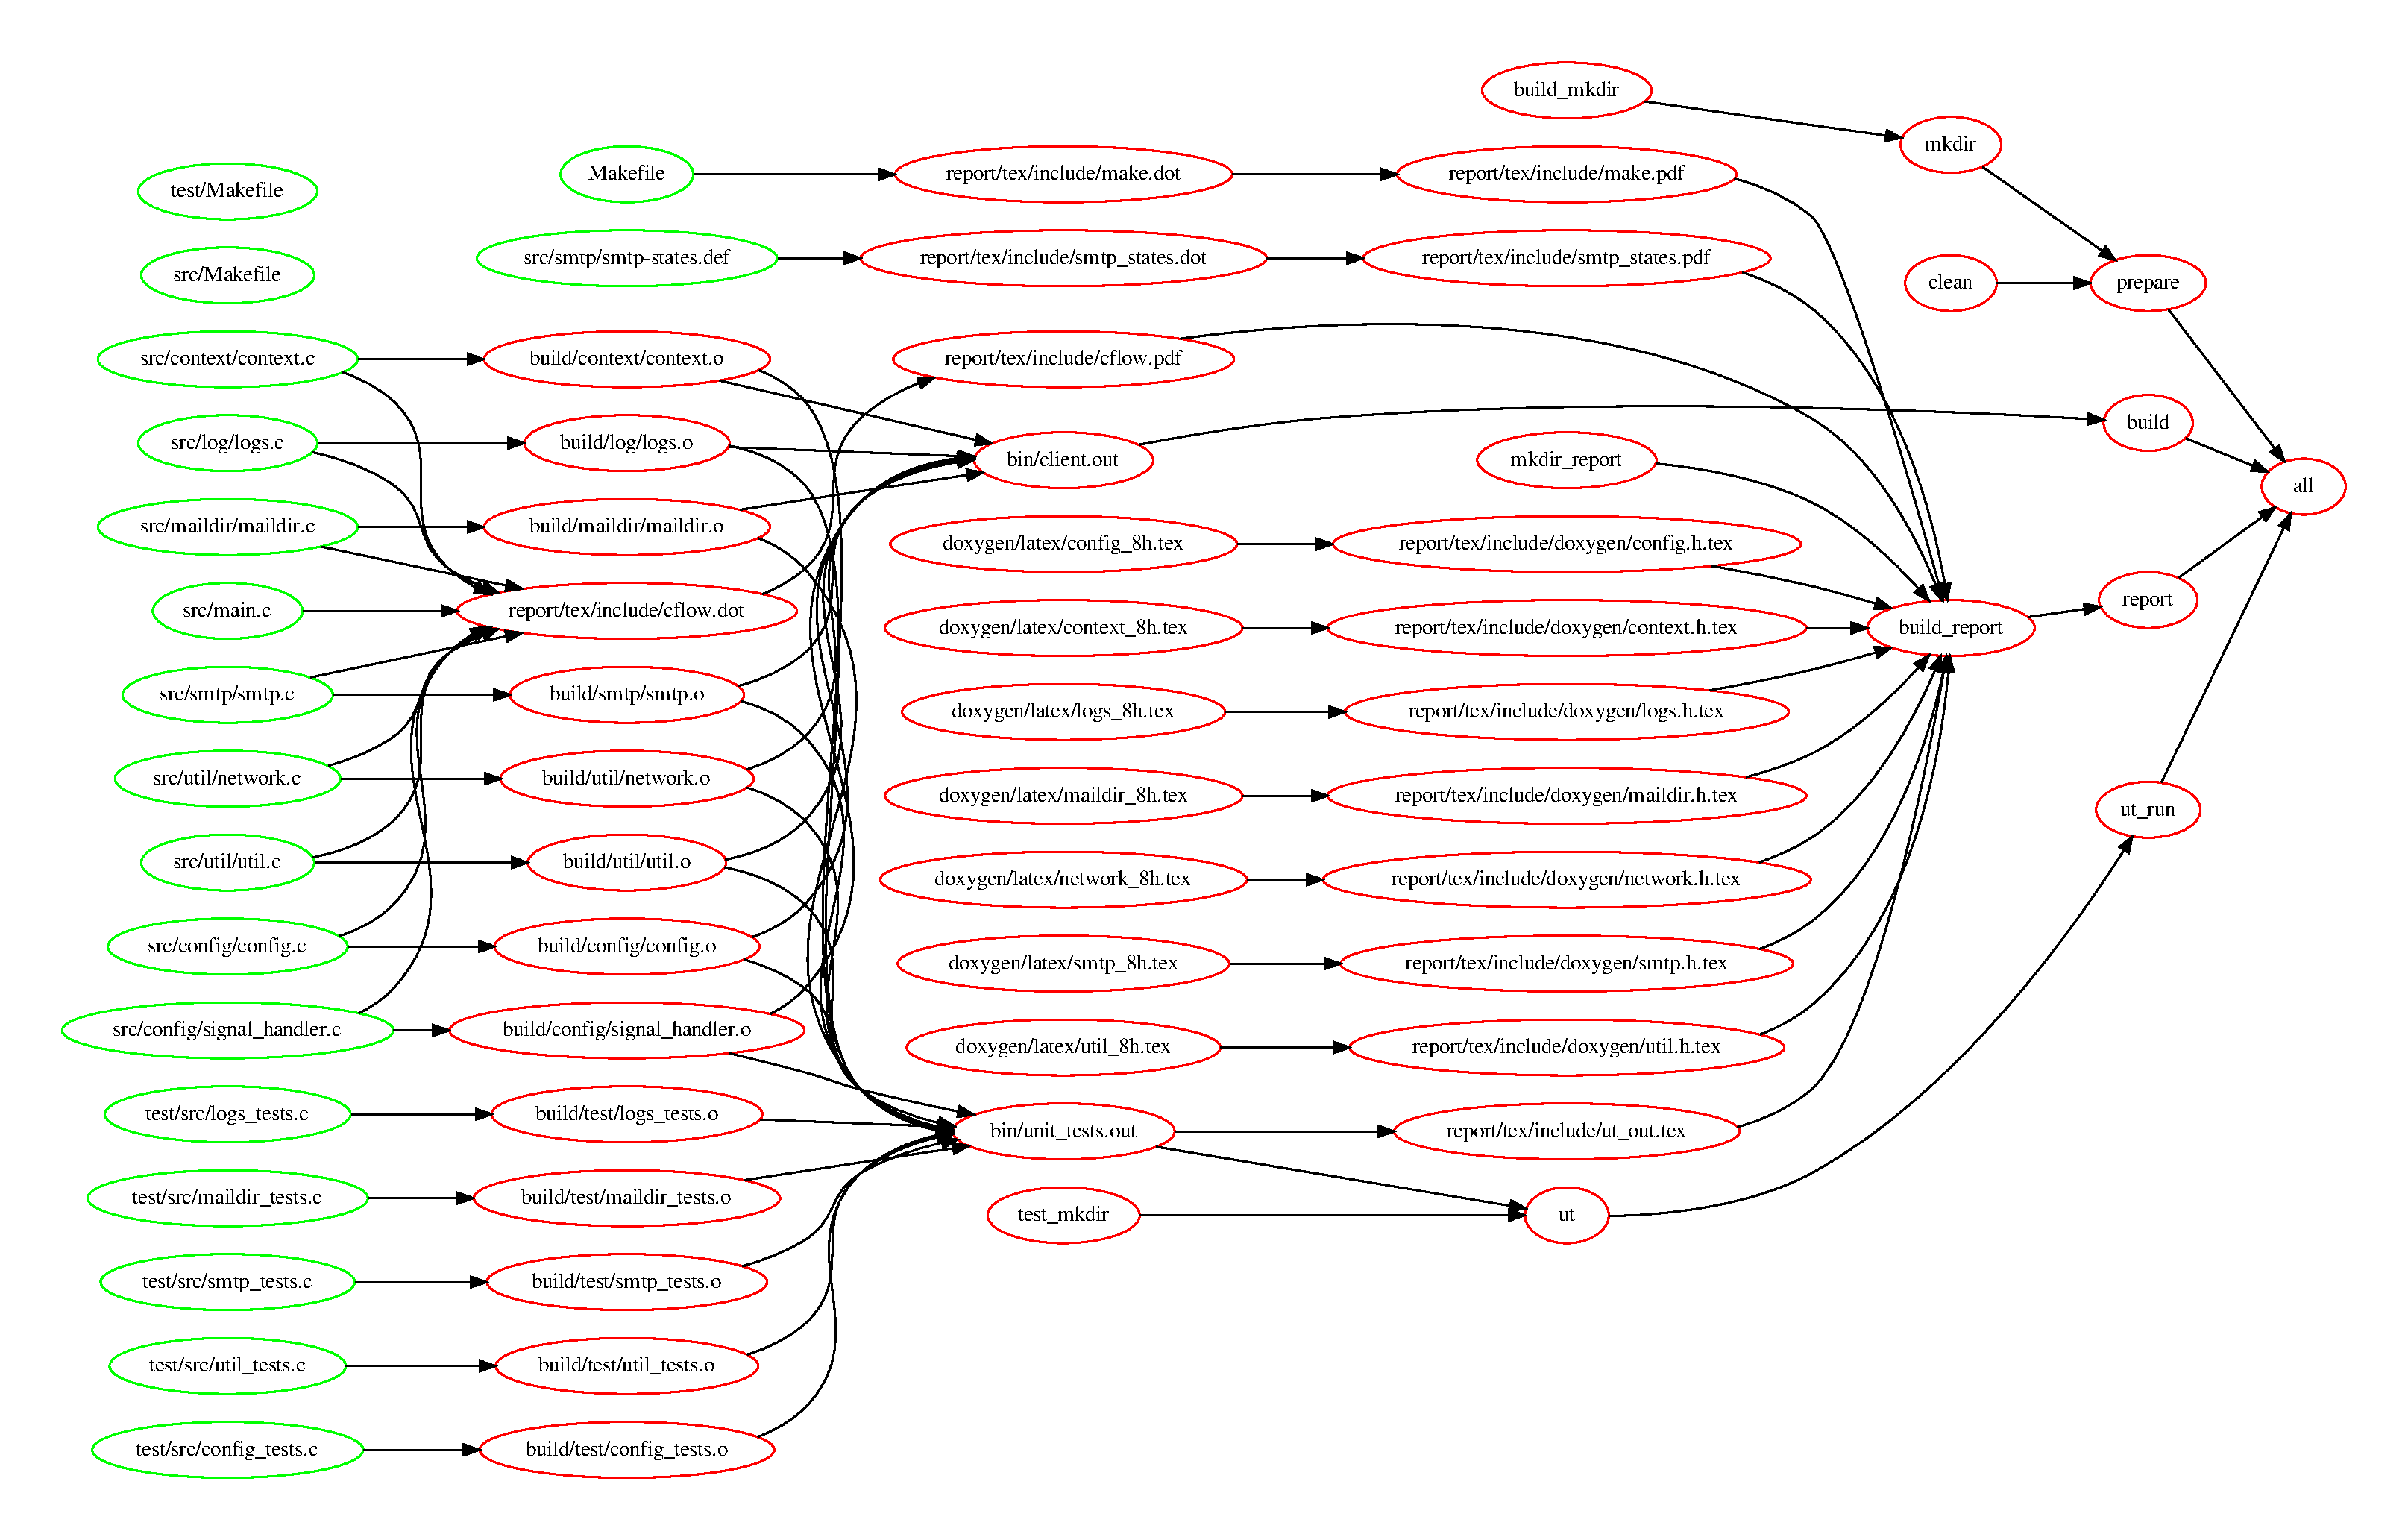
\includegraphics[width=\textwidth]{./include/make.pdf}
	\caption{Структура проекта.}
	\label{fig:make_server}
	\end{figure}

	
	\begin{figure}[H]
	\centering
	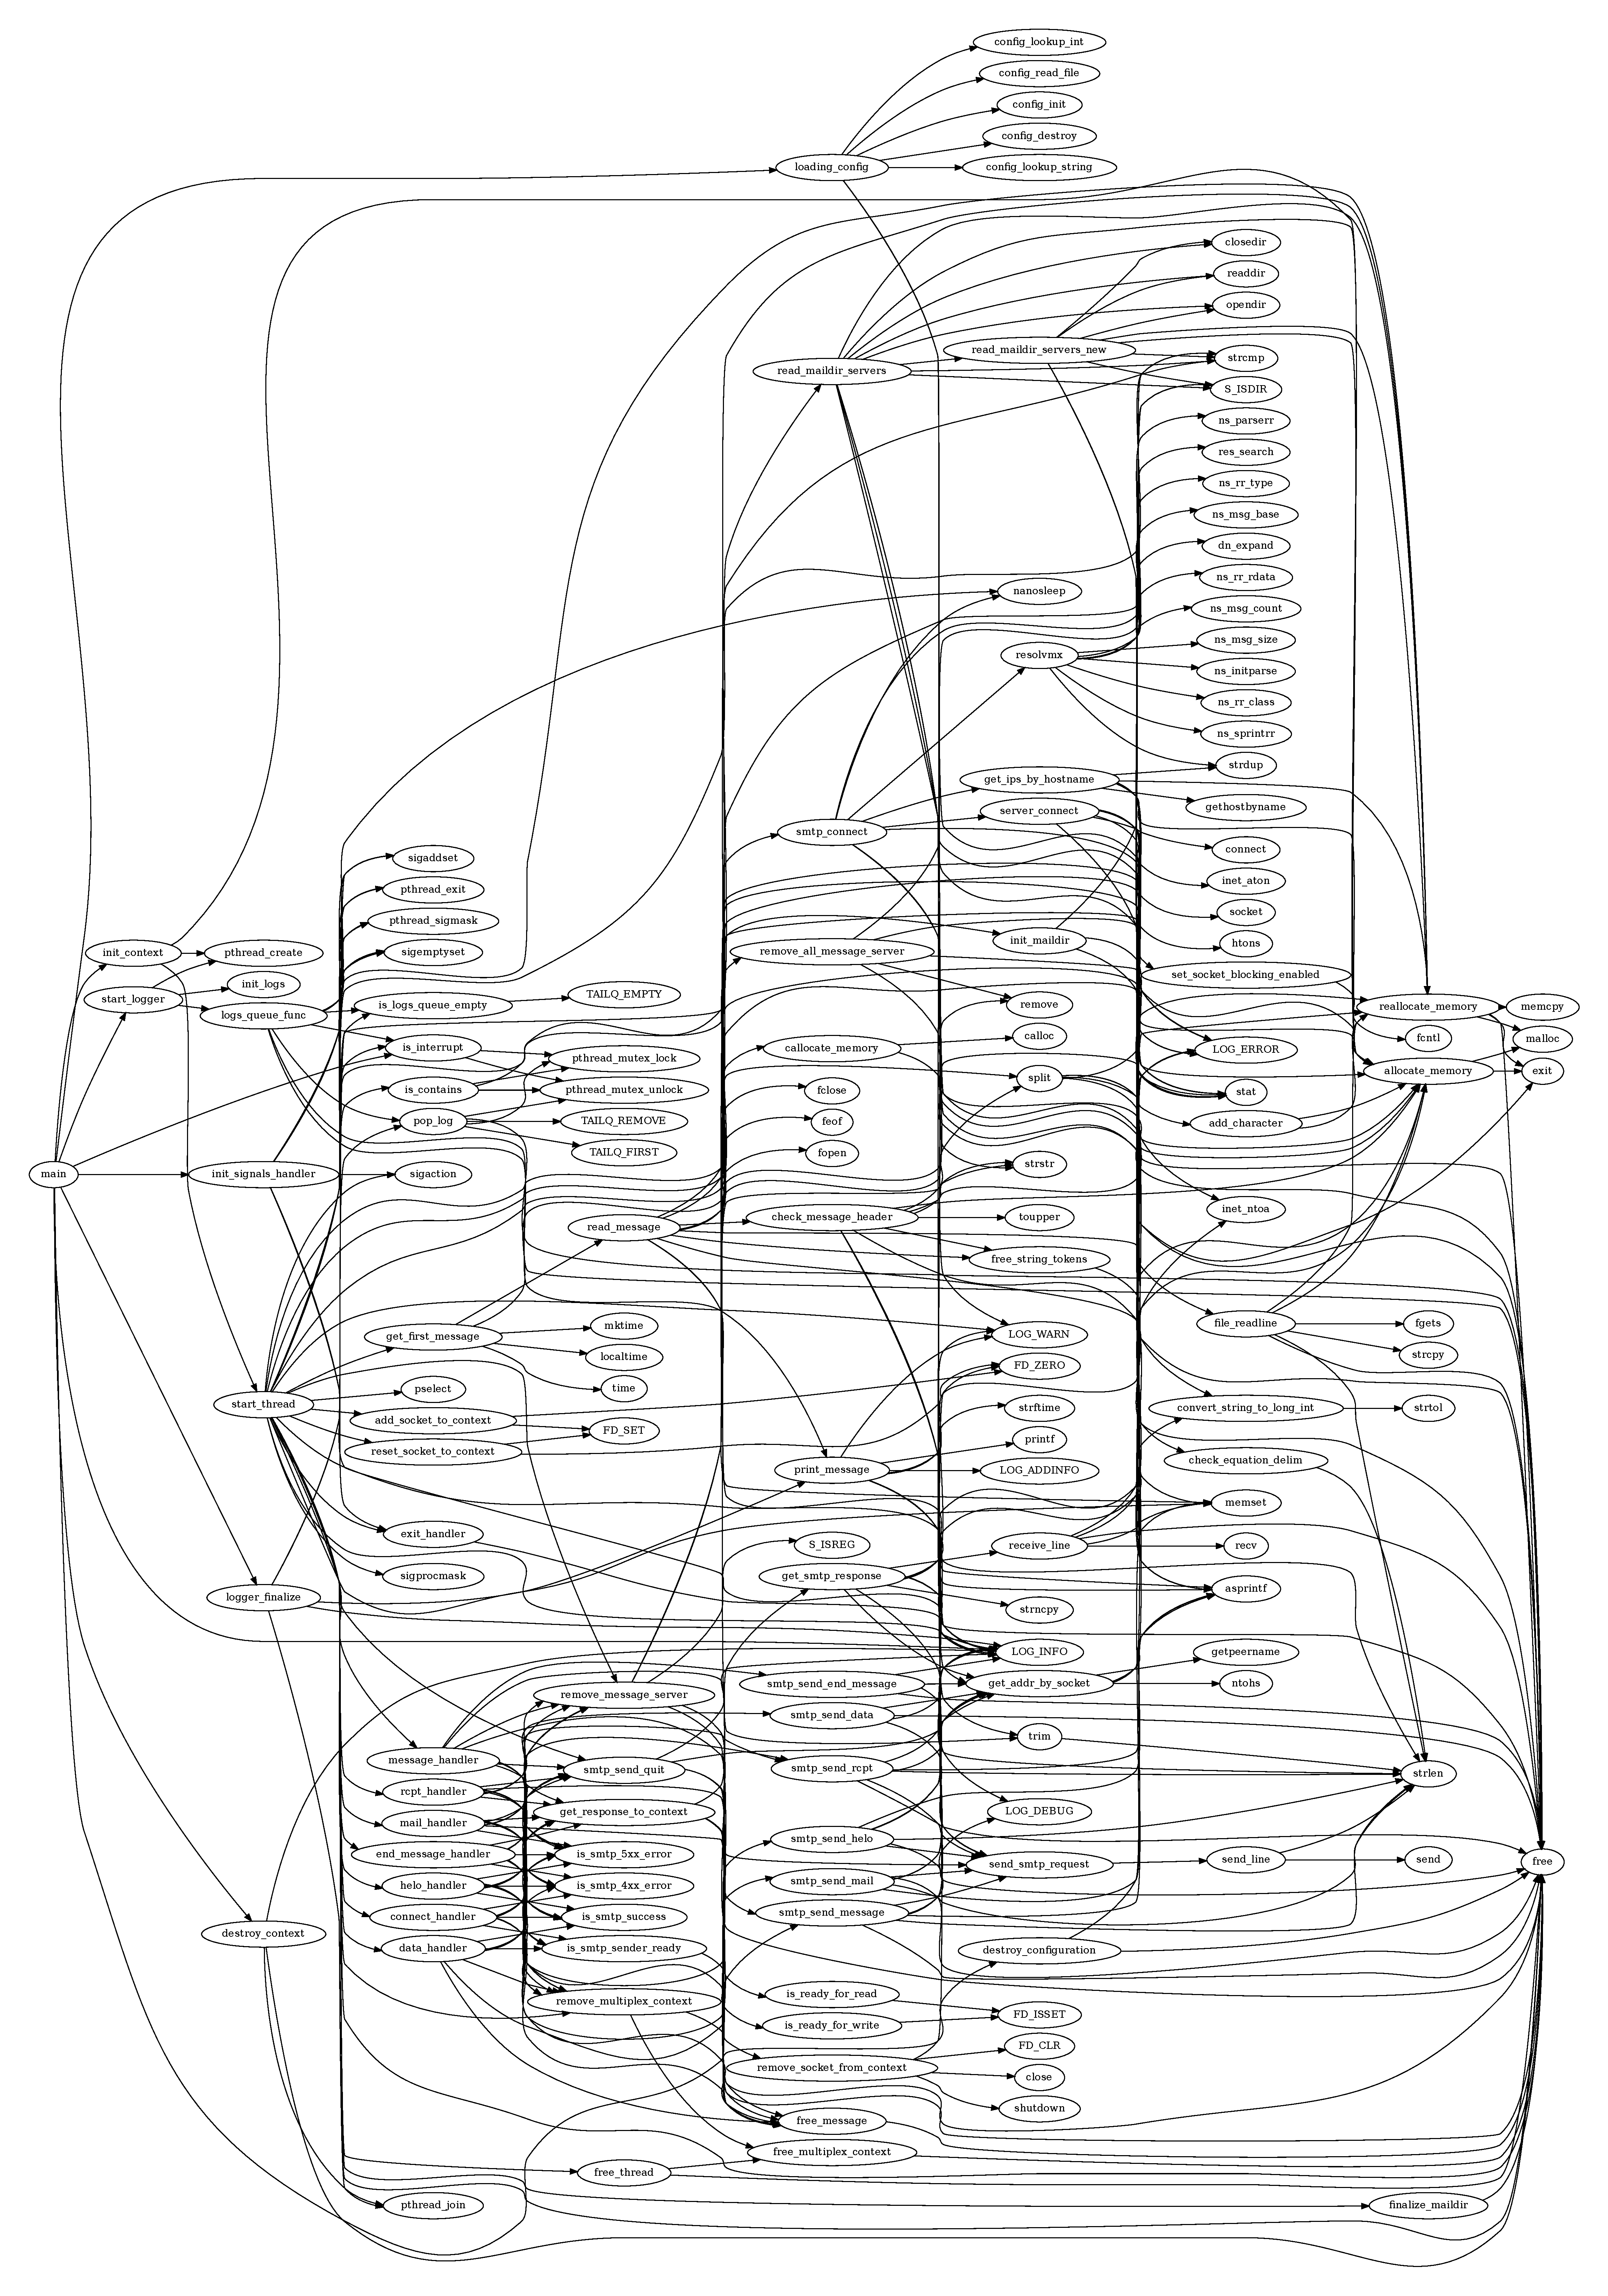
\includegraphics[width=\textwidth]{./include/cflow.pdf}
	\caption{Граф вызовов функций, который реализует всю логику.}
	\label{fig:cflow}
	\end{figure}


 \chapter{Технологический раздел}

	\section{Тестирование}
		Для тестирования отдельных модулей сервера, было написаны unit-тесты
		с использованием библиотеки cunit. Резултат работы тестиованяи представлен
		в листинге 
		\VerbatimInput{./include/unit_test_out.tex}
		\VerbatimInput{./include/valgrind_out.tex}
		
		Так же было реализовано интеграционное тестирование, на языке программирования python.

		Сценарии тестирований представлены в следующем листинге

		\VerbatimInput{../../test/server_auto_test/main.py}



		%\begin{landscape}
		%	\input{./include/lcov/index}
		%\end{landscape}
		%Отчет по покрытию тестами не строится в  gitlab!

\section{Основные функции программы}

Данный раздел  создан с помощью программы doxygen

\input{./include/doxygen/event_loop.h.tex}
\input{./include/doxygen/smtp_state.h.tex}
\input{./include/doxygen/smtp_state.h.tex}   
\input{./include/doxygen/maildir.h.tex}
\input{./include/doxygen/maildir_server.h.tex}
\input{./include/doxygen/maildir_user.h.tex}
\input{./include/doxygen/maildir_user.h.tex}	



	\addcontentsline{toc}{chapter}{Заключение}
	\chapter*{Заключение}
	В ходе выплнения курсовой работы был изучен протокол SMTP и реализовано серверное программное обеспечение выполняюще прием почты по данному протоколу. Для реализации конечного автомата протокола исопльзовалась утилита autofsm (autogen). При реализации сервера использовалась многопоточная архитектура и цикл событий, которые позволяют зарегистрировать множество обработчиков для некоторого набора событий, при этом множество возникших событий пареллельно обрабатываются в несокльких потоках путем вызова зарегистрированных обработчиков. Реализованное программное обеспечение было протестировано с помощью unit-тестирования с использованием бибилотеки cunit и интеграционного тестирования, которе было реализовано посредством языка программирования python.



	\printbibliography
	
	\newpage
	%\appendix
	%\section{A}\label{appendix:event_loop}
	% \begin{figure}[H]
    %\centering
  %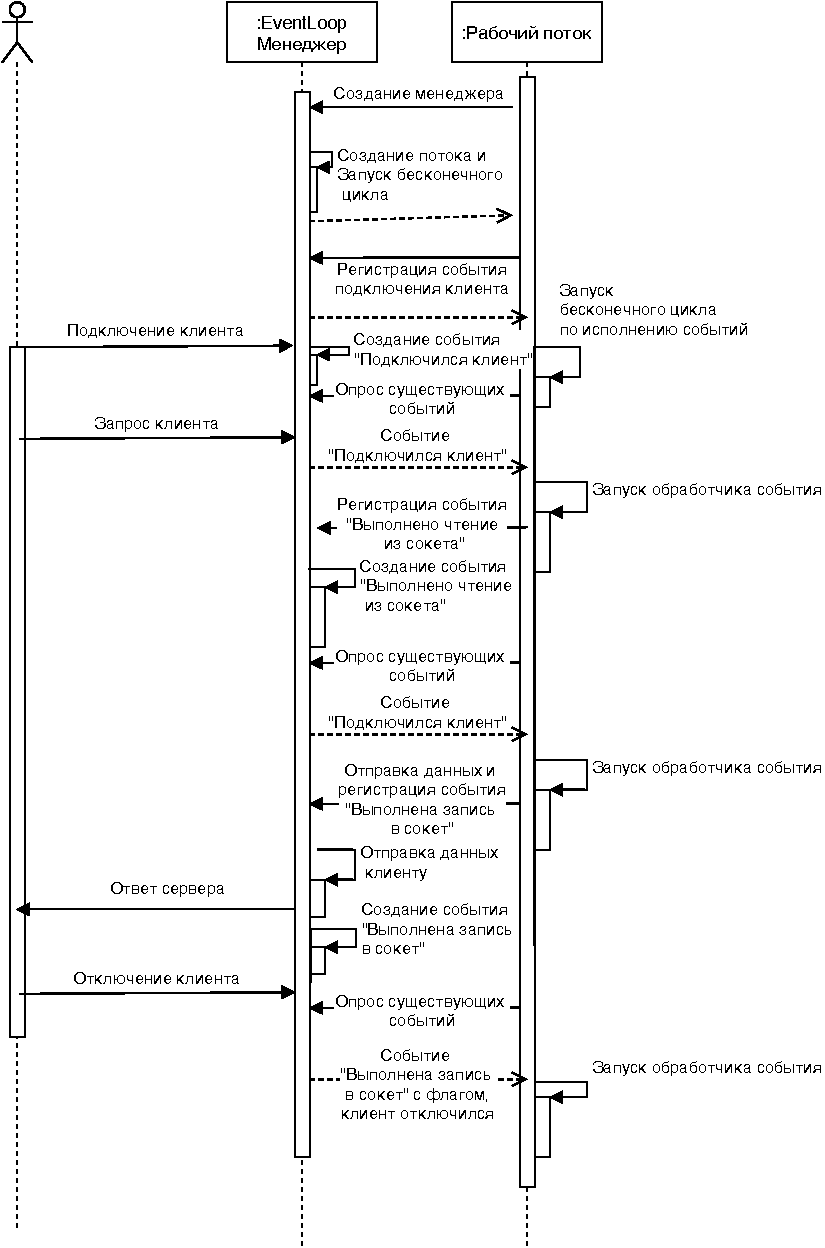
\includegraphics[scale=01]{./resource/SequenceDiagram_EventLoop.pdf}
%\end{figure}
 % Диграмма последовательности цикла событий сервера, описывающая подключение клиента, который отправлет запрос, ожидает ответ, а потом отключается. При отключении клиента, выставлется соответсвующий флаг, который обрабатывается в обработчике чтения из сокета или записи в сокет.
\end{document}